W~celu zweryfikowania czy zaimplementowane oprogramowanie działa poprawnie, wykonano zestaw testów. Sprawdzone zostało,
czy moduły komunikują się poprawnie między sobą (między modułami sieci oraz modułem MASTER a~modułem serwera sieciowego)
oraz czy dane, które moduł serwera sieciowego odebrał, wyświetlane są poprawnie na zaimplementowanej stronie
internetowej.

\section{\label{sect:test-network-comm}Testy komunikacji sieci} Do sprawdzenia poprawności komunikacji wewnątrz sieci
wykorzystana została implementacja funkcji, która zlicza ilość wysłanych zapytań przez moduł MASTER oraz ilość
otrzymanych odpowiedzi, oraz funkcja, która na podstawie otrzymanych wartości oblicza wartość procentową zapytań z~błędem
(niezależnie od tego, czy był to timeout -- przekroczenie czasu oczekiwania na odpowiedź, czy otrzymana odpowiedź nie
zgadzała się z~tą, na jaką moduł MASTER oczekiwał). Kod źródłowy odpowiedzialnych za to elementów przedstawiony został
na listingach \ref{lst:master-req-count} oraz \ref{lst:master-failedpercent}.

\lstinputlisting[
    language=C++,
    linerange={147-147,148-149,153-160,162-170},
    caption={Zliczanie całkowitej ilość zapytań oraz odpowiedzi zakończonych błędem (timeout, zły nagłówek odpowiedzi)},
    label={lst:master-req-count},
    float=htbp,
]{lora-psn/src/main.cpp}

\lstinputlisting[
    language=c++,
    linerange={242-249},
    caption={Implementacja funkcji pomocnicznej do wyznaczania wartości procentowej zapytań z~błędem},
    label={lst:master-failedpercent},
    float=htbp,
]{lora-psn/src/main.cpp}

Sieć została uruchomiona na pewien czas i~podczas jej pracy monitorowane było czy komunikacja działa poprawnie. Podczas
testu wykorzystano jedynie podgląd sieci poprzez monitor portu szeregowego na moduł MASTER. Na rys.
\ref{img:test-network-comm} przedstawiony został zrzut ekranu pokazujący, że sieć komunikuje się poprawnie oraz to, że
oprogramowanie zlicza całkowitą ilość zapytań oraz ilość błędów w~komunikacji wraz z~procentowym błędem.

\begin{figure}[!htbp]
    \centering
    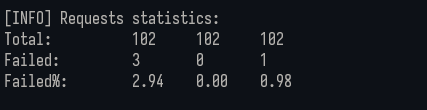
\includegraphics[width=0.65\textwidth]{screenshots/test-network-comm}
    \caption{\label{img:test-network-comm}Zrzut ekranu z~monitora portu szeregowego podczas testowania komunikacji
        w~sieci.}
\end{figure}

\FloatBarrier
\section{\label{sect:test-webserver-comm}Testy transmisji danych do serwera sieciowego} Wykonane zostały także testy
komunikacji modułu MASTER z~modułem serwera sieciowego. Sprawdzone zostało, czy dane zbierane przez sieć LoRa poprawnie
przesyłane przez magistralę I2C oraz dekodowane po stronie modułu serwera sieciowego.

Korzystając z~zaimplementowanego logowania przez port szeregowy modułu MASTER informacji o~transmisji przez magistralę
I2C (listing \ref{lst:main-transmitting}) oraz dodatkowej funkcjonalności w~module serwera sieciowego, której
implementacja przedstawiona została na listingu \ref{lst:webserver-count-transmission}, logującej przez port szeregowy
ilość odebranych transmisji, sprawdzona została poprawność komunikacji.

\lstinputlisting[
    language=c++,
    linerange={129-135},
    caption={Implementacja funkcjonalności zliczania transmisji z~modułu MASTER na module serwera sieciowego.},
    label={lst:webserver-count-transmission},
    float=htbp
]{feather-ws/src/main.cpp}

Moduły zostały uruchomione oraz włączone zostały monitor portu szeregowego modułu MASTER i~modułu serwera sieciowego.
Przez pewien czas prowadzona była obserwacja logowanych wartości. Podczas trwania testu stwierdzone zostało, że moduły
działają i~komunikują się poprawnie. Przykładowe logi, pokazujące poprawną komunikację przedstawione zostały na rys.
\ref{img:test-i2c-master} oraz \ref{img:test-i2c-webserver}.

\begin{figure}[!htbp]
    \centering
    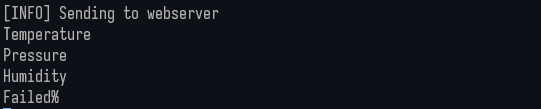
\includegraphics[width=0.70\textwidth]{screenshots/test-i2c-master}
    \caption{\label{img:test-i2c-master}Logi o~transmisji przez magistralę I2C z~modułu MASTER.}
\end{figure}

\begin{figure}[!htbp]
    \centering
    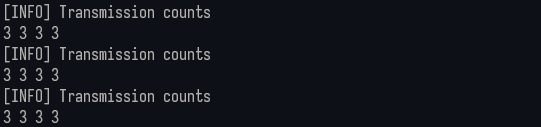
\includegraphics[width=0.70\textwidth]{screenshots/test-i2c-webserver}
    \caption{\label{img:test-i2c-webserver}Logi pokazujące poprawne odbieranie wartości z~magistrali I2C przez moduł
        serwera sieciowego.}
\end{figure}

\FloatBarrier
\section{\label{sect:test-webserver-website}Testy działania serwera sieciowego oraz strony internetowej} Ostatnim
wykonanym testem, który pozwolił na stwierdzenie, że zaimplementowane oprogramowanie działa poprawnie, było sprawdzenie
samego serwera sieciowego. Zweryfikowane zostało czy uruchamia się on poprawnie, gdy pojawi się możliwość zalogowania do
sieci lokalnej sieci Wi-Fi (której dane zostały podane w~pliku konfiguracyjnym) oraz czy poprawnie działa strona
internetowa, którą moduł serwuje użytkownikowi, chcącemu zobaczyć zebrane przez sieć LoRa dane.

Do testu wykorzystany został mobilny hotspot (lokalna sieć Wi-Fi utworzona przez smartphone) oraz zaimplementowana
rejestracja informacji o~logowaniu się modułu do sieci WiFi i~uruchamiania serwera sieciowego. Na rys.
\ref{img:wifi-hotspot} oraz \ref{img:webserver-wifi-logging} pokazane zostały włączony mobilny hotspot oraz logi
z~modułu serwera sieciowego. Na ich podstawie stwierdzone zostało, że serwer sieciowy działa poprawnie, ponieważ jednym
z~logów jest informacja o~starcie serwera z~jego lokalnym IP (umożliwiającym wyświetlenie strony internetowej) na porcie
80.

\begin{figure}[!htbp]
    \centering
    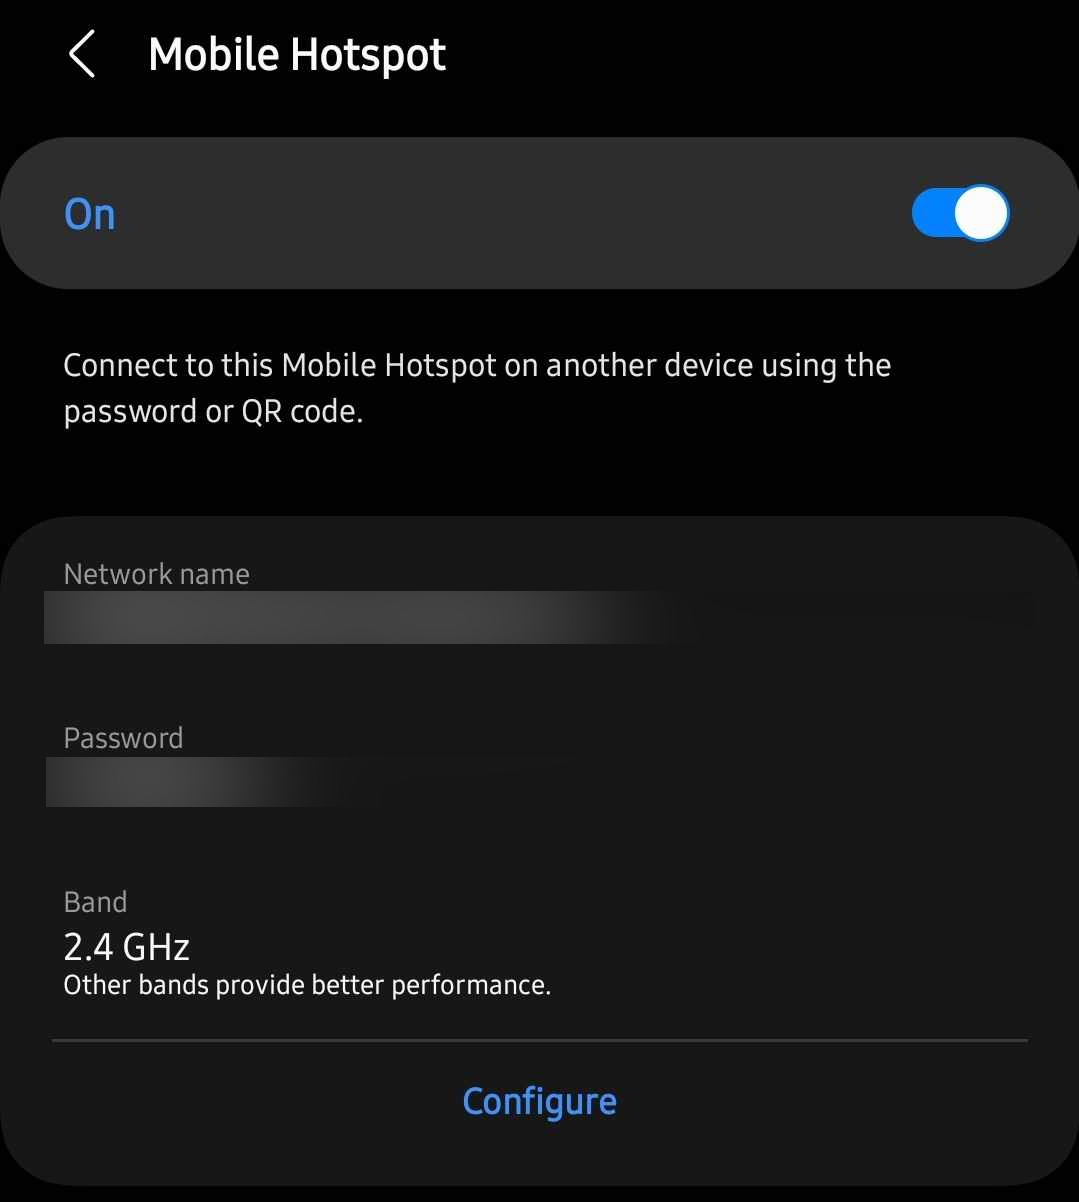
\includegraphics[width=0.50\textwidth]{screenshots/wifi-hotspot}
    \caption{\label{img:wifi-hotspot}Zrzut ekranu pokazujący włączony mobilny hotspot.}
\end{figure}

\begin{figure}[!htbp]
    \centering
    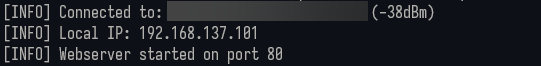
\includegraphics[width=0.70\textwidth]{screenshots/webserver-wifi-logging}
    \caption{\label{img:webserver-wifi-logging}Logi pokazujące poprawne połączenie z~siecią Wi-Fi oraz uruchomienie
        serwera sieciowego.}
\end{figure}

\FloatBarrier
Działanie zaimplementowanej strony internetowej sprawdzone zostało poprzez wykonanie próby załadowania jej w~dwóch
przypadkach: przed pierwszym przesłaniem danych z~sieci LoRa (lub tuż po restarcie modułu serwera sieciowego) oraz po
tym, jak dane zostały przesłane. Miało to na celu sprawdzenie, poza samym ładowaniem strony, także czy jej zawartość
zostanie poprawnie zaktualizowana, gdy z~modułu MASTER przesłane zostaną dane. Rys. \ref{img:website-pre-data} pokazuje
poprawnie załadowaną stronę przed przesłaniem danych z~sieci LoRa, natomiast rys. \ref{img:website-post-data} to zrzut
ekranu z~widoczną poprawną aktualizacją danych po odebraniu ich przez moduł serwera sieciowego.

\begin{figure}[!htbp]
    \centering
    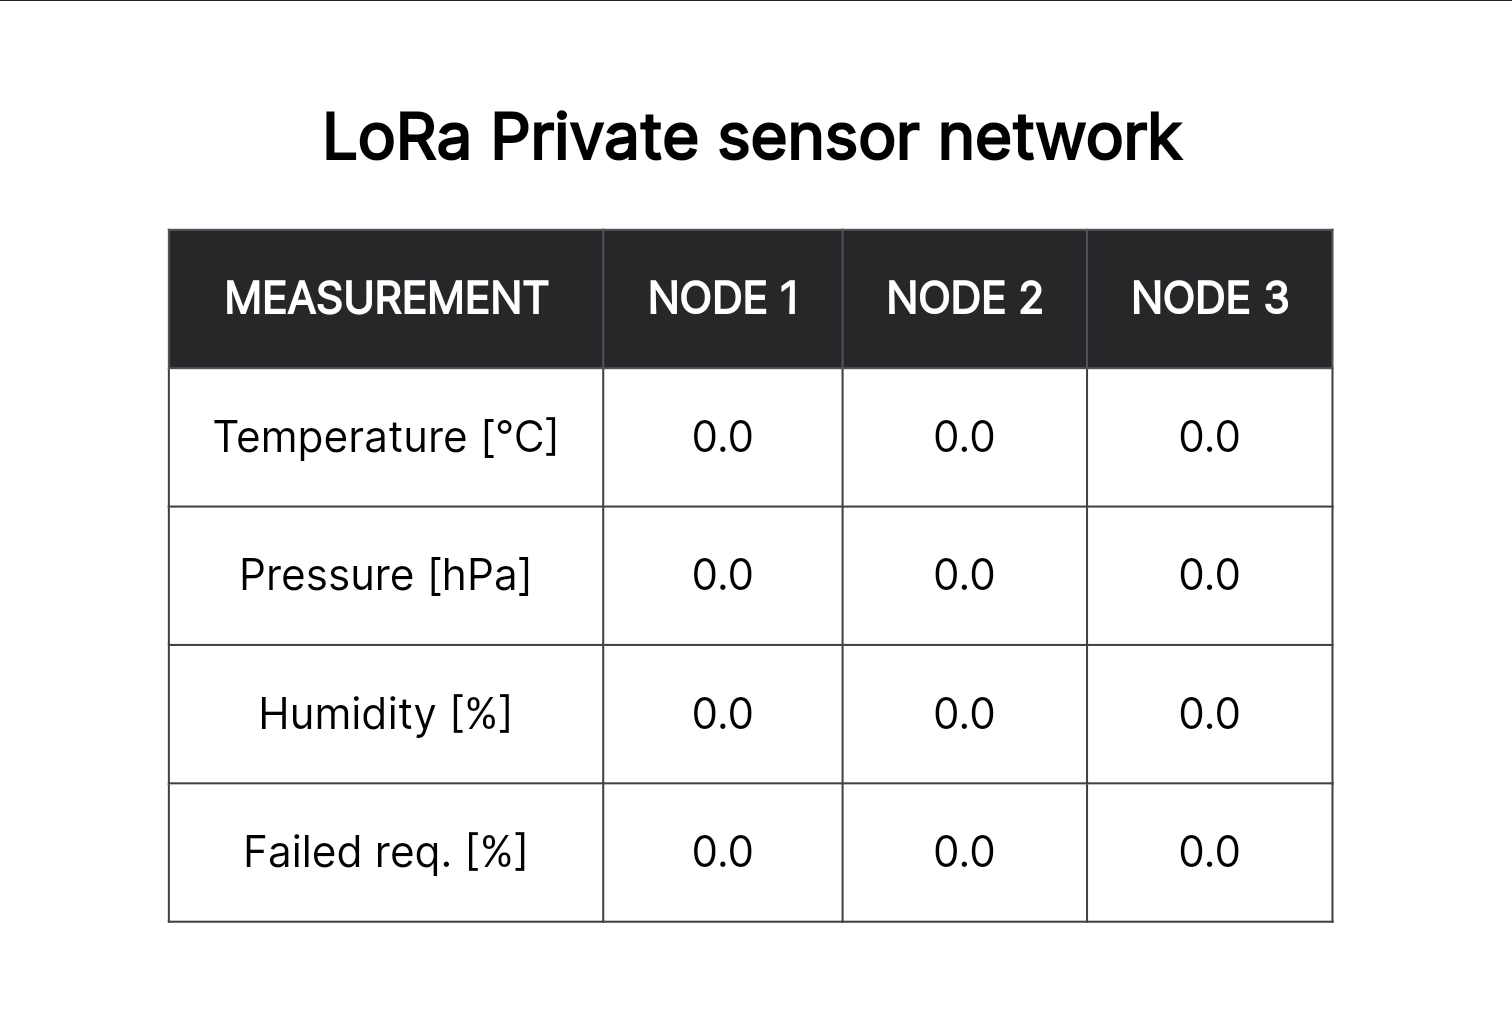
\includegraphics[width=0.65\textwidth]{screenshots/website-pre-data}
    \caption{\label{img:website-pre-data}Zrzut ekranu ze strony bez danych z~sieci.}
\end{figure}

\begin{figure}[!htbp]
    \centering
    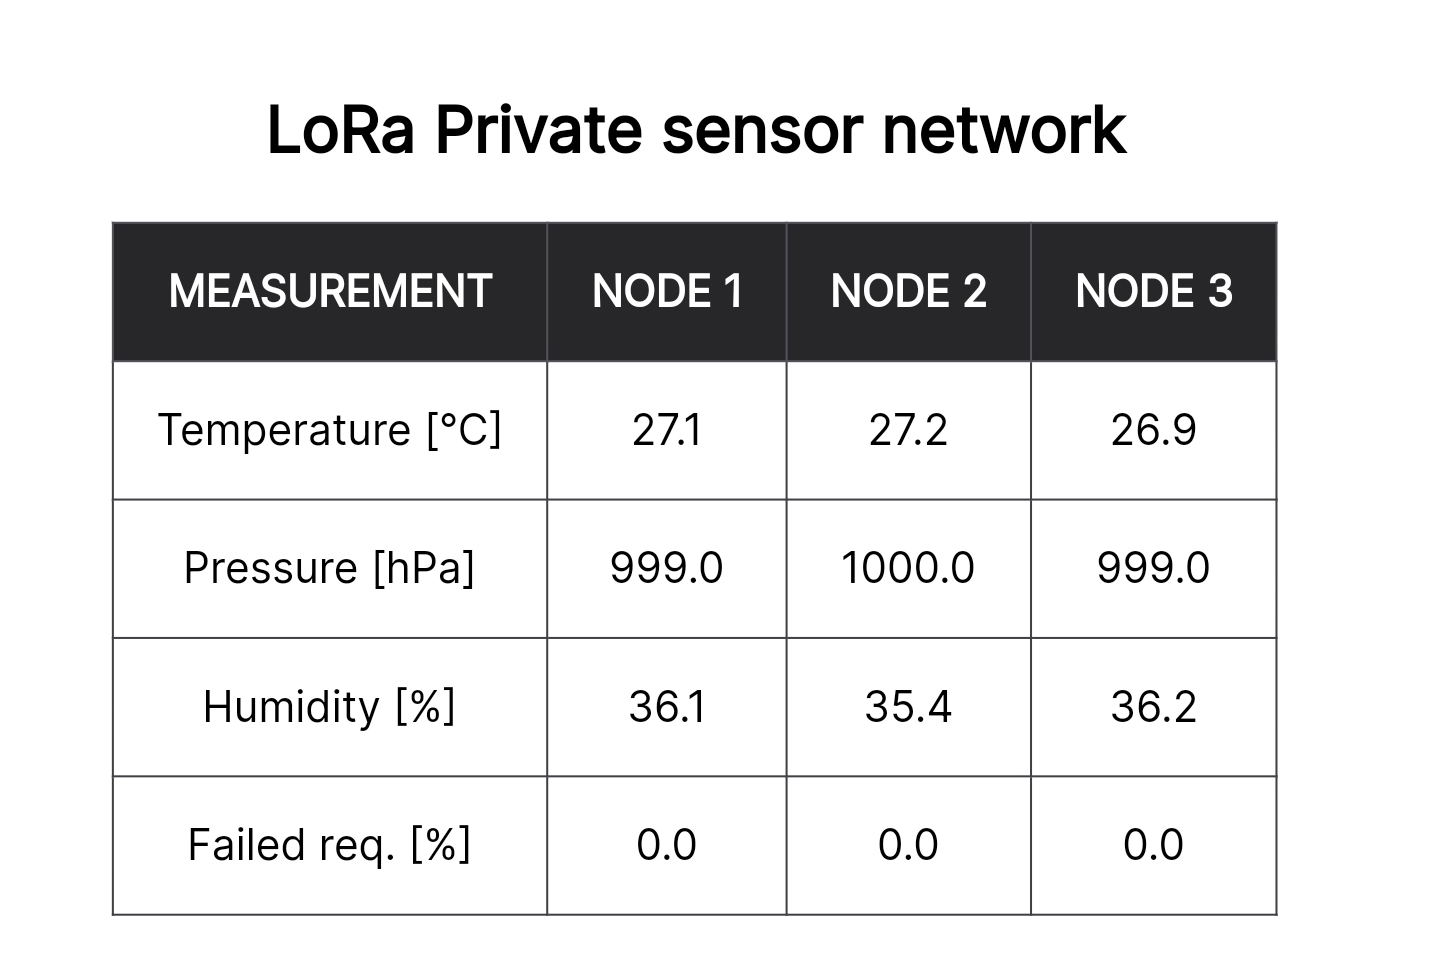
\includegraphics[width=0.65\textwidth]{screenshots/website-post-data}
    \caption{\label{img:website-post-data}Zrzut ekranu ze strony po otrzymaniu danych przez moduł serwera sieciowego.}
\end{figure}
